\label{sec:jeffery}
The Jeffery orbits describe the orientational motion of an ellipsoidal particle in Stokes flow. The general equations of motion for any ellipsoid in shear flow were found by Jeffery\cite{Jeffery} who also solved these equations of motion for axisymmetric ($a_1 \ne a_2 = a_3$) ellipsoidal particles. Solutions for asymmetric particles were found numerically by Yarin \emph{et al.}~\cite{Yarin} who also rewrote the equations in a different but equivalent form. The equations of rotational motion for a triaxial particle in shear flow are in the form of Yarin \emph{et al.}

\begin{subequations}\label{eq:jeffrey}
\begin{align}
\frac{d\theta}{dt} 	&= (g_2 \sin \psi + g_3 \cos \psi ) \sin \theta, \\
\frac{d\phi}{dt} 	&= \tfrac{1}{2} + g_3\sin \psi - g_2 \cos \psi,\\
\frac{d\psi}{dt}	&= g_1 + (g_2\cos \psi - g_3\sin \psi) \cos \theta. \\
\end{align}
\end{subequations}

\noindent The functions  $g_i$ are defined as

\begin{subequations}
\begin{align}
g_1 &= \frac{a_2^2 - a_3^2}{2(a_2^2 + a_3^2)} 
		\left(-\tfrac{1}{2}(\cos^2 \theta + 1 )\sin 2\phi \sin 2\psi + \cos\theta \cos 2\phi \cos 2\psi \right), \\
g_2 &= \frac{a_3^2 - a_1^2}{2(a_1^2 + a_3^2)}
		\left( -\cos\theta \sin 2\phi \sin\psi  +  \cos 2\phi \cos\psi \right), \\
g_3 &= \frac{a_1^2 - a_2^2}{2(a_1^2 + a_2^2)}
		\left( \cos\theta \sin 2\phi \cos\psi + \cos 2\phi \sin\psi \right).
\end{align}
\end{subequations}

\noindent Here $(\phi, \theta, \psi)$ are the Euler angles seen in Figure \ref{fig:eulerangles}. 
%Note that Yarin uses $a_x, a_y, a_z$ in place of $a_1, a_2, a_3$.

Note that the eq. (\ref{eq:jeffrey}) uses the coordinate system from Yarin \emph{et al.}\cite{Yarin} which differ from the one used in this thesis, details are discussed in Johansson \cite{AntonThesis}. Numerical solutions for three different initial conditions for an asymmetric particle are shown in Figure \ref{fig:orbitparams}.

\begin{figure}[H]
\centering
\begin{subfigure}[b]{0.45\textwidth}
\includegraphics[width=\textwidth]{figures/theory/map.pdf}
\caption{A poincare map}\label{fig:orbitmap}
\end{subfigure}\hspace{1em}%
\begin{subfigure}[b]{0.5\textwidth}
\includegraphics[width=\textwidth]{figures/theory/orbit.pdf}
\caption{The time series for the components \\ of the unit vector.}\label{fig:orbitparams}
\end{subfigure}
\caption{A Poincare map and three different orbits for a simulated particle with $\lambda=7$ and $\epsilon=0.05$. The three orbits highlight the three different kinds of motion, the quasi-periodic sign changing orbit in blue, the quasi-periodic sign preserving orbit in red and the periodic orbit in green. We see that while $n_x$ and $n_y$ look qualitatively similar but differ in amplitude for the different orbits, $n_z$ shows three different types of behaviour}
\label{fig:orbittypes}
\end{figure}



Looking at Figure \ref{fig:orbitparams} we see that $n_x$ and $n_y$ are periodic, corresponding to periodic rotation around the $z$-axis. We refer to these rotations as flips. The period $\eta$ of $n_x$ and $n_y$ is for an axisymmetric particle \cite{Jeffery}

\begin{equation}\label{eq:flipRate}
\eta = 2\pi \left( \lambda + \frac{1}{\lambda} \right)\frac{1}{\kappa},
\end{equation}

\noindent where $\kappa$ is the shear rate. 

The time evolution of $\theta$ and $\psi$ for different initial conditions can be plotted in a Poincaré map, also known as a Surface-of-Section (S.O.S.)~\cite{poincare}. This plots the $\psi$ and $\theta$ coordinates each time $\phi = 0$. The successive points on the Poincaré map for each initial condition move and explore certain regions of the surface of section. This region is referred to as the \emph{orbit}. 

For a particle with an asymmetry $\epsilon$ in the range $\left[0.01-0.05\right]$ there are three classes of orbits, depending on the initial condition $\theta_0$.

\begin{enumerate}
\item \textbf{Periodic}: $\left|\theta_0\right| \approx 1$ in which there is little variation and the particle is largely periodic with fluctuations too small to measure.
\item \textbf{Quasi-periodic sign preserving}: For $\left|\theta_0\right|> \theta_b$ the amplitude of $\cos(\theta)$ changes noticeably but does not change sign. Here $\theta_b$ is a breaking point that changes for different $\epsilon$.
\item \textbf{Quasi-periodic sign changing}: For small $\left|\theta_0\right| < \theta_b$ the amplitude of $\cos(\theta)$ changes noticeably and changes sign. 
\end{enumerate}

Simulations of these three different types of orbits for a particle with $\lambda=7$ and $\epsilon=0.05$ are illustrated in Figure \ref{fig:orbittypes}. Figure \ref{fig:orbittypes} shows the orbits on the S.O.S. and Figure \ref{fig:orbitparams} shows the components of $\mathbf{n}$ as a function of time. We can see that while $n_x$ and $n_y$ are periodic, albeit with different amplitudes, the  behaviour of $n_z$ is significantly different for the different orbits. The $n_z \approx 1$  orbit shown in green is constant on the S.O.S and is simply periodic over time. The sign preserving quasi-periodic orbit in red is bent on the S.O.S. We can see in the time series that it is doubly periodic as it peaks with a fixed period but the amplitude of the peaks vary periodically themselves. The sign changing quasi-periodic orbit in blue also peaks periodically with varying peak amplitude but these also change sign, again with a fixed period.


For larger asymmetries $\epsilon > 0.05$ there are chaotic orbits that explore a larger region of the S.O.S. The simulations used do not have long enough time evolutions for the chaotic orbits to fill the regions in the way that quasi-periodic or periodic orbits fill the one dimensional regions that define their orbits. This results in the chaotic orbits appearing as a 'sea' of dots instead of filled lines. Chaotic orbits can been seen around the quasi-periodic sign changing orbits in Figure \ref{fig:orbitmap4}.

\begin{figure}[H]
\centering
\begin{subfigure}[3a]{0.40\textwidth}
\includegraphics[width=\textwidth]{figures/theory/7-1-1.pdf}
\caption{Poincare map for $\lambda = 7, \epsilon = 0$.}\label{fig:orbitmap1}
\end{subfigure}\hspace{1em}%
\begin{subfigure}[3b]{0.40\textwidth}
\includegraphics[width=\textwidth]{figures/theory/7-1o01-1.pdf}
\caption{Poincare map for $\lambda = 7, \epsilon = 0.01$.}\label{fig:orbitmap2}
\end{subfigure} \\
\begin{subfigure}[3a]{0.40\textwidth}
\includegraphics[width=\textwidth]{figures/theory/7-1o05-1.pdf}
\caption{Poincare map for $\lambda = 7, \epsilon = 0.05$.}\label{fig:orbitmap3}
\end{subfigure}\hspace{1em}%
	\begin{subfigure}[3b]{0.40\textwidth}
\includegraphics[width=\textwidth]{figures/theory/7-1o25-1.pdf}
\caption{Poincare map for $\lambda = 7, \epsilon = 0.25$.}\label{fig:orbitmap4}
\end{subfigure} 
\caption{Four Poincare maps for different $\epsilon$. Already at $\epsilon = 0.01$ there are noticeably quasi-periodic 
orbits around the centre at $\cos(\theta) \approx \psi \approx 0$ but it is also a significantly larger region for $\epsilon = 0.05$. For $\epsilon = 0.25$ we can see chaotic orbits surrounding the circular orbits in the centre that appear as a 'sea' of dots.} %q Note that some wavelike pattern can appear to exist in the figure \ref{fig:orbitmap2} and  \ref{fig:orbitmap2}, this is caused by aliasing/compression issues with printing several curved lines close together.}\label{fig:orbitmaps}
\end{figure}

\subsection{Winding number} \label{sec:winding}
The quasi-periodic orbits are also referred to as doubly-periodic~\cite{Yarin}. They are called doubly-periodic to emphasize the fact that the amplitude of a short period $\theta_2$ also varies periodically with a longer period $\theta_1$. The ratio between the two periods is referred to as the winding number $\omega$ referring to the winding around a unit torus. The shorter period $\theta_2$ corresponds to rotations around the small cross section of the unit torus and the longer period $\theta_1$ corresponds to rotations around the large circumference of the torus. The winding number is the fraction of these periods, as is shown in Figure \ref{fig:torus}. 

\begin{figure}[H]
\begin{center}
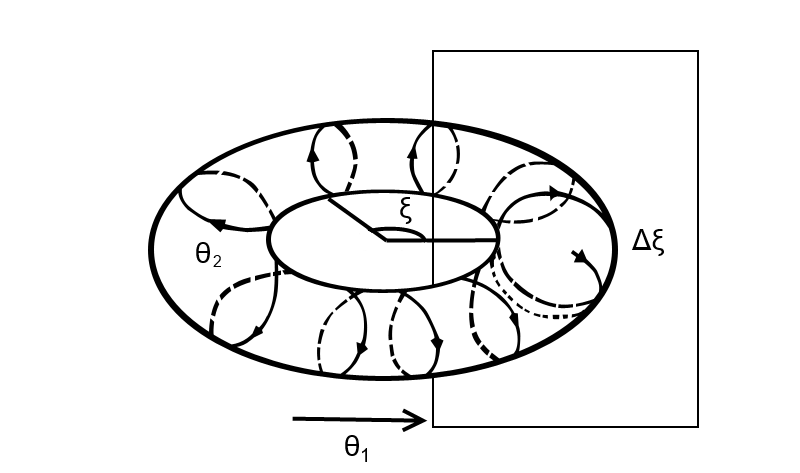
\includegraphics[width=0.5\textwidth]{figures/theory/torus.png}
\end{center}
\caption{Winding around a unit torus with period $\theta_1$ around the large circumference and $\theta_2$ around the small cross section. The offset after one rotation around the large circumference $\theta_1 / \theta_2$ is called the winding number. This figure idea was taken from Schuster \cite{introchaos}}
\label{fig:torus}
\end{figure}

\noindent The winding number is defined as \cite{introchaos}

\begin{equation}
\omega_{def}  = \lim\limits_{n \rightarrow \infty} \frac{f^n(\xi) - \xi_0}{n}.
\end{equation}

where $\xi$ is the angle around the large circumference of the torus and $f^n(\xi)$ is the shift caused in $n$ rotations around the smaller axis. 
Applying this to our double-periodic orbits $\xi$ would be the angle with period $\theta_1$ and $n$ the number of flips with period $\theta_2$. 
Since we cannot measure $\xi$ I consider it more comprehensible to consider the inverse winding number: The number of flips necessary to 
complete one period of $\xi$. This can be measured as is shown in Figure \ref{fig:windingDef}. If we measure over several $\theta_1$ peaks the average winding number approximates the real one. We refer to the this inverse winding number as $\omega$ and it is given by

\begin{equation}\label{eq:winding}
\omega = \frac{\theta_1}{\theta_2}.
\end{equation}

\noindent The winding number of the quasi-periodic sign preserving orbit from Figure \ref{fig:orbittypes} and the way we approximate $\theta_1$ (and thereby $\omega$) is illustrated in Figure \ref{fig:windingDef}.

\begin{figure}[H]
\begin{center}
\includegraphics[width=0.7\textwidth]{figures/theory/WindingNrFixed2.pdf}
\end{center}
\caption{The quasi-periodic sign preserving orbit from Figure \ref{fig:orbitparams} over a longer time, highlighting the short period $\theta_2$ which is simply the period of $\phi$ and the longer period $\theta_1$. We find the inverse winding number as the ratio between the longer and shorter periods.}
\label{fig:windingDef}
\end{figure}

%This can also be thought of as the number of intersections on the surface of section before coming back to the initial condition, divided by the number of laps. A lap for a circular orbit is a rotation around the center whereas for a flat orbit it is moving along length of the orbit. asdasd, see figure MAKE A FIGURE. 
The winding number is the same for any point along a quasi-periodic orbit on a Poincaré map but it is different for different orbits as well as for different asymmetries. The winding numbers for orbits along $\psi=0$ for $\epsilon=\{0.01, 0.05, 0.10\}$ can be seen in Figure \ref{fig:windingdifferent}. The difference in winding number between the different $\epsilon$ for the sign changing orbits are almost a factor 2. This means that if we can measure the winding number for a sign changing orbit it allows us to approximate the asymmetry of the particle even though the variation in $n_z$ are identical. Without looking at the winding number we cannot determine if a particle with an orbit close to $n_z = 0$ and small variations in amplitude is close to symmetric or not.
 
\begin{figure}[H]
\begin{center}
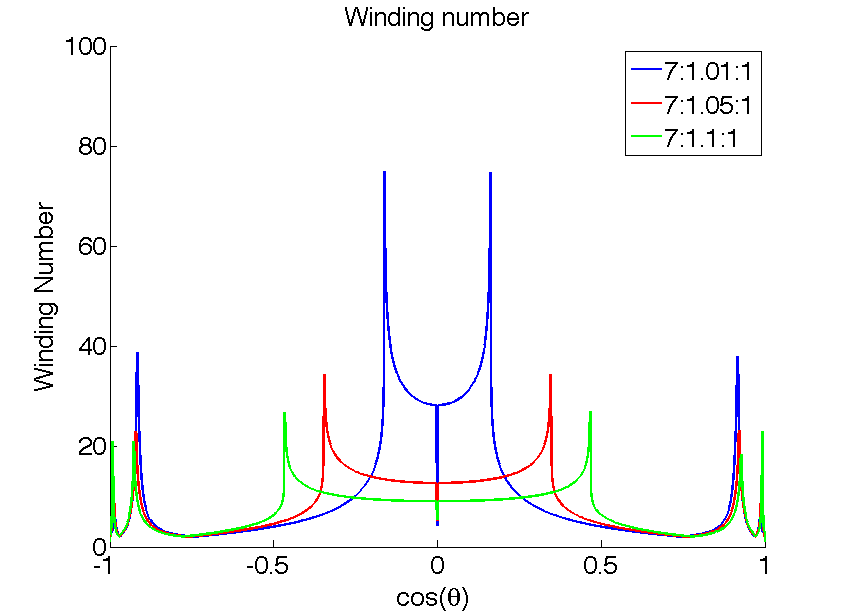
\includegraphics[width=0.7\textwidth]{figures/theory/WindingTrend.png}
\end{center}
\caption{The winding number for $\psi_0 = 0$ and $\lambda = 7$ as a function of $\cos(\theta_0)$ for three different asymmetries, $\epsilon = 0.01$, $\epsilon = 0.05$ and $\epsilon = 0.10$. The sharp edge that occurs at different points for the different asymmetries, but centred around zero, is where the sign changing orbits end and sign preserving orbits begin, denoted by $\theta_b$. We see that a lower asymmetry leads to a sharper difference between the sign changing and the sign preserving orbits and that higher asymmetry in general leads to lower winding numbers on average.}
\label{fig:windingdifferent}
\end{figure}
